\documentclass{article}
\usepackage{amsmath} % aligned env

\usepackage{relsize} % make some math large
\usepackage{bm} % make some math bold

\usepackage{caption}
\usepackage{geometry}
\geometry{
	a4paper,
	noheadfoot=true,
	left=1.0in,
	right=1.0in,
	top=1.0in,
	bottom=1.0in,
}

\usepackage{tikz}
\usetikzlibrary{decorations.pathreplacing}

\definecolor{myLightGray}{RGB}{191,191,191}
\definecolor{myGray}{RGB}{160,160,160}
\definecolor{myDarkGray}{RGB}{144,144,144}
\definecolor{myDarkRed}{RGB}{167,114,115}
\definecolor{myRed}{RGB}{255,58,70}
\definecolor{myGreen}{RGB}{0,255,71}

\begin{document}

\title{Latex Tikz Examples, Timeline Charts}
\author{\href{https://fanwangecon.github.io/}{Fan Wang}\thanks{https://fanwangecon.github.io, repository: \href{https://fanwangecon.github.io/Tex4Econ/}{Tex4Econ}}}
\date{\today}

\section{Tikz Example 1}

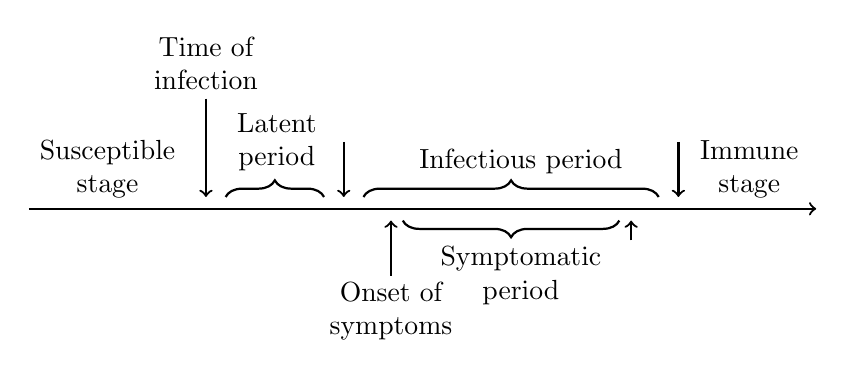
\begin{tikzpicture}[scale=1]
\node[align=center] at (1,0.5) {Susceptible\\stage};
\node[align=center] at (2.25,1.85) {Time of\\infection};
\draw [thick,->] (2.25,1.4) -- (2.25,0.15);
\node[align=center] at (3.15,0.85) {Latent\\period};
\draw [thick,decorate,decoration={brace,amplitude=6pt,raise=0pt}] (2.5,0.15) -- (3.75,0.15);
\draw [thick,->] (4,0.85) -- (4,0.15);
\node[align=center] at (6.25,0.6) {Infectious period};
\draw [thick,->] (8.25,0.85) -- (8.25,0.15);
\node[align=center] at (9.15,0.5) {Immune\\stage};
\draw [thick,decorate,decoration={brace,amplitude=6pt,raise=0pt}] (4.25,0.15) -- (8,0.15);
\draw [thick,->] (0,0) -- (10,0);
\draw [thick,->] (4.6,-0.85) -- (4.6,-0.15);
\draw [thick,->] (7.65,-0.4) -- (7.65,-0.15);
\draw [thick,decorate,decoration={brace,amplitude=6pt,raise=0pt,mirror}] (4.75,-0.15) -- (7.5,-0.15);
\node[align=center] at (6.25,-0.85) {Symptomatic\\period};
\node[align=center] at (4.6,-1.3) {Onset of\\symptoms};
\end{tikzpicture}

\section{Tikz Example 2}

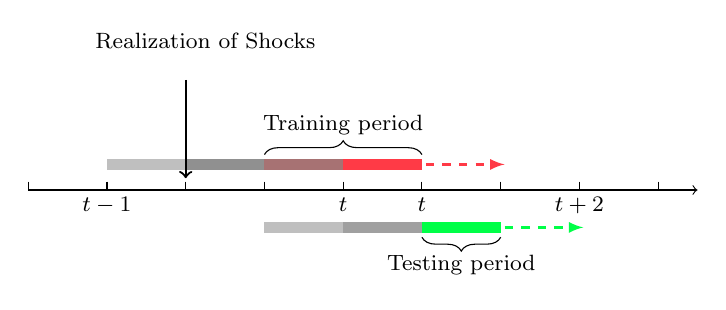
\begin{tikzpicture}[%
    every node/.style={
        font=\footnotesize,
        text height=1ex,
        text depth=.25ex,
    },
]
% draw horizontal line
\draw[->] (0,0) -- (8.5,0);

% draw vertical lines
\foreach \x in {0,1,...,8}{
    \draw (\x cm,3pt) -- (\x cm,0pt);
}

% place axis labels
\node[anchor=north] at (1,0) {$t-1$};
\node[anchor=north] at (4,0) {$t$};
\node[anchor=north] at (5,0) {$t$};
\node[anchor=north] at (7,0) {$t+2$};

% draw scale above
\fill[myLightGray] (1,0.25) rectangle (2,0.4);
\fill[myDarkGray] (2,0.25) rectangle (3,0.4);
\fill[myDarkRed] (3,0.25) rectangle (4,0.4);
\fill[myRed] (4,0.25) rectangle (5,0.4);
\draw[myRed,dashed,thick,-latex] (5.05,0.325) -- (6.05,0.325);

% draw scale below
\fill[myLightGray] (3,-0.4) rectangle (4,-0.55);
\fill[myGray] (4,-0.4) rectangle (5,-0.55);
\fill[myGreen] (5,-0.4) rectangle (6,-0.55);
\draw[myGreen,dashed,thick,-latex] (6.05,-0.475) -- (7.05,-0.475);

% draw curly braces and add their labels
\draw[decorate,decoration={brace,amplitude=5pt}] (3,0.45) -- (5,0.45)
    node[anchor=south,midway,above=4pt] {Training period};
\draw[decorate,decoration={brace,amplitude=5pt}] (6,-0.6) -- (5,-0.6)
    node[anchor=north,midway,below=4pt] {Testing period};

% Add Lines
\node[align=center] at (2.25,1.85) {Realization of Shocks};
\draw [thick,->] (2,1.4) -- (2,0.15);

\end{tikzpicture}

\section{Tikz Example 3}

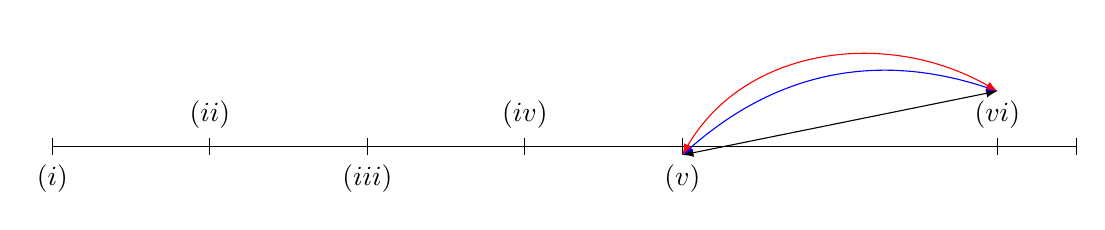
\begin{tikzpicture}
\draw (0,0) -- (13,0);
\foreach \x in {0,2,4,6,8,12,13}
  \draw (\x cm,3pt) -- (\x cm,-3pt);
\draw (0,0) node[below=3pt] (a) {$(i)$} node[above=3pt] {};
\draw (2,0) node[below=3pt] (b) {} node[above=3pt] {$(ii)$};
\draw (4,0)  node[below=3pt]  {$(iii)$} node[above=3pt] (c) {};
\draw (6,0) node[below=3pt](d) {} node[above=3pt] {$(iv)$};
\draw (8,0) node[below=3pt](e) {$(v)$} node[above=3pt] {};
\draw (12,0) node[above=3pt] (f) {$(vi)$} node[below=3pt] {};
\draw[latex-latex]
  (e.north) -- (f.north);
\draw[latex-latex,blue]
  (e.north) to[bend left] (f.north);
\draw[latex-latex,red]
  (e.north) to[out=60,in=150] (f.north);
\end{tikzpicture}\qquad

\section{Tikz Example 4}

\begin{tikzpicture}
\draw (0,0) -- (13,0);
\foreach \x in {0,2,4,6,8,12,13}
  \draw (\x cm,3pt) -- (\x cm,-3pt);
\draw (0,0) node[below=3pt] (a) {$(i)$} node[above=3pt] {};
\draw (2,0) node[below=3pt] (b) {} node[above=3pt] {$(ii)$};
\draw (4,0)  node[below=3pt]  {$(iii)$} node[above=3pt] (c) {};
\draw (6,0) node[below=3pt](d) {} node[above=3pt] {$(iv)$};
\draw (8,0) node[below=3pt](e) {$(v)$} node[above=3pt] {};
\draw (12,0) node[above=3pt] (f) {$(vi)$} node[below=3pt] {};
\draw[latex-latex]
  (e.north|-f.north) -- (f.north);
\draw[latex-latex,blue]
  (e.north|-f.north) to[bend left] (f.north);
\draw[latex-latex,red]
  (e.north|-f.north) to[out=60,in=120] (f.north);
\end{tikzpicture}

\section{Tikz With Caption}

\begin{figure}[!ht]
\centering
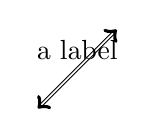
\begin{tikzpicture}[object/.style={thin,double,<->}]
  \draw[object] (7cm,-1cm) -- (6cm,-2cm) node[midway,above] {a label};
\end{tikzpicture}
\caption{A caption.}
\end{figure}

\section{Tikz Timeline}

\subsection{Tikz Timeline Plain}
%%%%%%%%%%%%%%%%%%%%%%%%%%%%%%%%%%%%%%%%%%%%%%%
%%% Model Timeline
%%%%%%%%%%%%%%%%%%%%%%%%%%%%%%%%%%%%%%%%%%%%%%%

\begin{figure}[h]
  \begin{minipage}{1\linewidth}
  \caption{Model Timeline}
  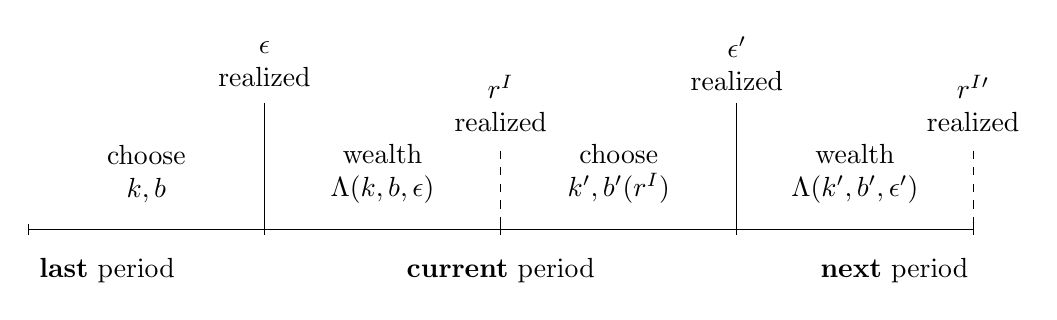
\begin{tikzpicture}
  \draw (0,0) -- (12,0);
  \foreach \x in {0,3,6,9,12}
    \draw (\x cm,2pt) -- (\x cm,-2pt);
  % Last Period
  \node[align=center] at (1.5, 0.7) {choose \\ $k, b$ };
  % Current Period
  \node[align=center] at (3, 2.1)  (a) {$ \epsilon$ \\ realized};
  \draw [thin, -] (3, 1.6) -- (3, 0);
  \node[align=center] at (4.5, 0.7) (b) {wealth  \\ $\Lambda(k,b, \epsilon)$ };
  \node[align=center] at (6, 1.6)  (a) {$ r^I$ \\ realized};
  \draw [thin, dashed] (6, 1.0) -- (6, 0);
  \node[align=center] at (7.5, 0.7) {choose \\ $k^{\prime}, b^{\prime}(r^I)$ };
  % Next Period
  \node[align=center] at (9, 2.1) {$ \epsilon^{\prime}$ \\ realized};
  \draw [thin, -] (9, 1.6) -- (9, 0);
  \node[align=center] at (10.5, 0.7) {wealth  \\ $\Lambda(k^{\prime}, b^{\prime}, \epsilon^{\prime})$ };
  \node[align=center] at (12, 1.6)  (a) {$ r^{I\prime}$ \\ realized};
  \draw [thin, dashed] (12, 1.0) -- (12, 0);
  % Text Below
  \draw (1,0) node[below=7pt] {\textbf{last} period};
  % \draw [thick,decorate,decoration={brace,amplitude=6pt,raise=0pt,mirror}] (2.8,-0.30) -- (8.8,-0.30);
  \draw (6,0)  node[below=7pt]  {\textbf{current} period};
  \draw (11,0) node[below=7pt] {\textbf{next} period};
  % % Arrows
  % \draw[latex-latex,blue]
  %   (a.north|-b.north) to[out=60,in=120] (b.north);
  % \draw[latex-latex,red]
  %   (e.north|-f.north) to[out=60,in=120] (f.north);
  \end{tikzpicture}
  {\footnotesize
  \emph{Notes:} (1) $k$, the risky capital choice, is determined before productivity shock $\epsilon$ realization. (2) $b^{\prime}$, the net financial choice including principle and interests owed, is determined given $r^I$, which is the interest rate cost of informal loan taken out this period.}
  \end{minipage}
  \end{figure}

  \subsection{Tikz Timeline with Skeleton Tree}
  %%%%%%%%%%%%%%%%%%%%%%%%%%%%%%%%%%%%%%%%%%%%%%%
  %%% Model Timeline With Tree Inside
  %%%%%%%%%%%%%%%%%%%%%%%%%%%%%%%%%%%%%%%%%%%%%%%

  \tikzset{
      % Two node styles for game trees: solid and hollow
      solid node/.style={circle,draw,inner sep=1.5,fill=black},
      hollow node/.style={circle,draw,inner sep=1.5,fill=white}
  }

  \def\famm{15mm}
  \def\height{2}
  \tikzstyle{level 1}=[level distance=\famm,sibling distance=\famm]
  \tikzstyle{level 2}=[level distance=\famm,sibling distance=\famm]

  \begin{figure}[h]
    \begin{minipage}{1\linewidth}
    \caption{Model Timeline With Tree Inside}
    \begin{tikzpicture}
    \draw (0,0) -- (12,0);
    \foreach \x in {0,2,4,12}
      \draw (\x cm,2pt) -- (\x cm,-2pt);
    % Last Period
    \node[align=center] at (1, 0.7) {choose \\ $k, b$ };
    % Current Period
    \node[align=center] at (2, 2.1)  (a) {$ \epsilon$ \\ realized};
    \draw [thin, -] (2, 1.6) -- (2, 0);
    \node[align=center] at (3, 0.7) (b) {wealth  \\ $\Lambda(k,b, \epsilon)$ };
    \node[align=center] at (4, 1.6)  (a) {$ r^I$ \\ realized};
    \draw [thin, dashed] (4, 1.0) -- (4, 0);
    \node[solid node, align=center, label=left:{$P1$}]  at (6, 1.5) {}
    [grow=right]
    child
    child{
        [grow=right]
        child
        child{
            [grow=right]
            child
            child
            child
            child
            }
        child
        }
    child;
    % Next Period
    \node[align=center] at (12, 2.1) {$ \epsilon^{\prime}$ \\ realized};
    \draw [thin, -] (12, 1.6) -- (12, 0);
    % Text Below
    \draw (1,0) node[below=7pt] {\textbf{last} period};
    \draw (6,0) node[below=7pt]  {\textbf{current} period};
    % % Arrows
    % \draw[latex-latex,blue]
    %   (a.north|-b.north) to[out=60,in=120] (b.north);
    % \draw[latex-latex,red]
    %   (e.north|-f.north) to[out=60,in=120] (f.north);
    \end{tikzpicture}
    {\footnotesize
    \emph{Notes:} (1) $k$, the risky capital choice, is determined before productivity shock $\epsilon$ realization. (2) $b^{\prime}$, the net financial choice including principle and interests owed, is determined given $r^I$, which is the interest rate cost of informal loan taken out this period.}
    \end{minipage}
    \end{figure}

\subsection{Tikz Timeline with Spanning and Annotated Tree}
  %%%%%%%%%%%%%%%%%%%%%%%%%%%%%%%%%%%%%%%%%%%%%%%
  %%% Model Timeline With Fancy Tree Inside
  %%%%%%%%%%%%%%%%%%%%%%%%%%%%%%%%%%%%%%%%%%%%%%%

  \def\famm{20mm}
  \def\height{2}
  \tikzstyle{level 1}=[level distance=\famm,sibling distance=\famm]
  \tikzstyle{level 2}=[level distance=\famm,sibling distance=\famm]

  \begin{figure}[h]
    \begin{minipage}{1\linewidth}
    \caption{Model Timeline with Fancy Tree Inside}
    \begin{tikzpicture}
    \draw (0,0) -- (12,0);
    \foreach \x in {0,2,4,12}
      \draw (\x cm,2pt) -- (\x cm,-2pt);
    % Last Period
    \node[align=center] at (1, 0.7) {choose \\ $k, b$ };
    % Current Period
    \node[align=center] at (2, 2.1)  (a) {$ \epsilon$ \\ realized};
    \draw [thin, -] (2, 1.6) -- (2, 0);
    \node[align=center] at (3, 0.7) (b) {wealth  \\ $\Lambda(k,b, \epsilon)$ };
    \node[align=center] at (4, 1.6)  (a) {$ r^I$ \\ realized};
    \draw [thin, dashed] (4, 1.0) -- (4, 0);

    \node(0)[solid node, align=center, % solid node gives fist (left to right) black dot
    label=left:{
       $\textcolor{black}{\mathlarger{\mathlarger{\mathlarger{\bm{\phi}}}}}$
        }] at (5.75, 1.5) {}
    [grow=right]
    child{
    [black] node(11)[]{}
    edge from parent
          node[sloped, below, black]{$\phi=0$}
    }
    child{
    [grow=right]
    % The starting node for theta
    node(12)[solid node, xshift=16, yshift=0, % solid node gives second (left to right) black dot
                    label=left:{
                      $\textcolor{black}{\mathlarger{\mathlarger{\mathlarger{\bm{\theta}}}}}$
                    }]{}
    % Draw the theta branches
      child{
          [red] node(21)[]{}
          edge from parent
              node[sloped, below, black]{$\theta=0$}
      }
      child{
          [white] node(22)[xshift=16, yshift=0]{}
          edge from parent
              [draw=none] % prevents a line to be drawn from phi to phi
              node[above, black, xshift=7]{$k' = \theta \cdot \Lambda$}
              node[below, black, xshift=10]{$b' = \Lambda - k'$}
      }
      child{
          [black] node(23)[]{}
          edge from parent
              node[sloped, above, black]{$\theta=1$}
      }
    edge from parent
      [draw=none] % prevents a line to be drawn from phi to phi
      % node[above, black, yshift=-55]{$c = \phi \cdot \Gamma$}
      % node[below, black, yshift=-55]{$\Lambda = \left(1-\phi\right) \cdot \Gamma$}
      node[above, black, xshift=4]{$c = \phi \cdot \Gamma$}
      node[below, black, xshift=4]{$\Lambda = \Gamma - c$}
      }
    child{
    [red] node(13)[]{}
    edge from parent
          node[sloped, above, black]{$\phi=1$}
    };
    \draw[dashed, bend right]
    (11) to (13);
    \draw[dashed, bend right]
    (21) to (23);
    % Next Period
    \node[align=center] at (12, 2.1) {$ \epsilon^{\prime}$ \\ realized};
    \draw [thin, -] (12, 1.6) -- (12, 0);
    % Text Below
    \draw (1,0) node[below=7pt] {\textbf{last} period};
    \draw (6.5,0) node[below=7pt]  {\textbf{current} period, $\Lambda$ realized, choose $k'$ and $b'$};
    % % Arrows
    % \draw[latex-latex,blue]
    %   (a.north|-b.north) to[out=60,in=120] (b.north);
    % \draw[latex-latex,red]
    %   (e.north|-f.north) to[out=60,in=120] (f.north);
    \end{tikzpicture}
    {\footnotesize
    \emph{Notes:} (1) $k$, the risky capital choice, is determined before productivity shock $\epsilon$ realization. (2) $b^{\prime}$, the net financial choice including principle and interests owed, is determined given $r^I$, which is the interest rate cost of informal loan taken out this period.}
    \end{minipage}
    \end{figure}

\section{Tikz Timeline Frame}

\subsection{Empty Frame}

\def\fgw{1.0*\textwidth}
\def\fgh{0.20*\textheight}

\newcommand{\tikzframe}{
	\draw (0,     \fgh) -- (\fgw,     \fgh);
	\draw[loosely dotted] (0, 0.5*\fgh) -- (\fgw, 0.5*\fgh);
	\draw (0, 0       ) -- (\fgw, 0       );
	% Three Straight Lines
	\draw[dashed] (0.125*\fgw, 0  ) -- (0.125*\fgw,   \fgh);
	\draw[dotted] (0.500*\fgw, 0.2*\fgh ) -- (0.500*\fgw,   0.8*\fgh);
	\draw[dashed] (0.875*\fgw, 0  ) -- (0.875*\fgw,   \fgh);

	\node[align=center] at (0.065*\fgw, 0.900*\fgh) {last\\period};
	\node[align=center] at (0.500*\fgw, 0.900*\fgh) {current period};
	\node[align=center] at (0.935*\fgw, 0.900*\fgh) {next\\period};

	\node[align=center] at (0.325*\fgw, 0.100*\fgh) {shocks and \\ income realization};
	\node[align=center] at (0.675*\fgw, 0.100*\fgh) {asset choices};
}
\newcommand{\tikzframebelowtext}[4]{
  \def\fgiw{#1*\textwidth}
  \def\fgih{#2*\textheight}
  \def\fgiwm{#3*\fgiw}
  \def\fgihm{#4*\fgih}

  % left pane middle point, align horizontally middle pane
  \def\fgiwlm{0.125*\textwidth + \fgiwm*0.5 - 0.5*0.125*\textwidth}
  % right pane middle point, align horizontally middle in pane
  \def\fgiwrm{\fgiwm + \fgiw*0.5 - 0.125*\textwidth*0.5 - \fgiwm*0.5}

  % fgihtb: figure internal height top pane bottom
  % bottom 10 percent space of top pane space
  \def\fgihtb{\fgihm + \fgih*0.085 - \fgihm*0.085}


  % There is a flow line on top, limited text
  % three parts, left prior, right after, middle current.
  % current in two parts, shock realization and choices.
  % In top part, span charts, simple text
  % in bottom part, sufficient height to allow for detailed text
  % descriptions.

  % Bottom and top lines
  \draw [solid] (0, \fgih) -- (\fgiw, \fgih);
  \draw [solid] (0, 0    ) -- (\fgiw, 0    );

  % Left and right lines
  \draw [solid] (0,     0) -- (0,     \fgih);
  \draw [solid] (\fgiw, 0) -- (\fgiw, \fgih);

  % verticle middle line
  \draw [solid] (\fgiwm, 0) -- (\fgiwm,   \fgih);
  % horizontal middle line (divide text and flow)
  \draw [solid] (0, \fgihm) -- (\fgiw,   \fgihm);

  % left border last period
  \draw[dashed] (0.125*\fgiw, 0  ) -- (0.125*\fgiw,   \fgih);
  % right border next period
  \draw[dashed] (0.875*\fgiw, 0  ) -- (0.875*\fgiw,   \fgih);

  % %
  % \draw[loosely dotted] (0, 0.575*\fgih) -- (\fgiw, 0.575*\fgih);
  % \draw[loosely dotted] (0, 0.350*\fgih) -- (\fgiw, 0.350*\fgih);

  \node[align=center] at (0.065*\fgiw, 0.900*\fgih) {last\\period};
  \node[align=center] at (0.500*\fgiw, 0.900*\fgih) {current period};
  \node[align=center] at (0.935*\fgiw, 0.900*\fgih) {next\\period};

  \node[align=center] at (\fgiwlm, \fgihtb) {shocks};
  \node[align=center] at (\fgiwrm, \fgihtb) {asset choices};
}


100 percent frame with 20 percent page height and 100 percent page width:

\begin{center}
\begin{tikzpicture}[scale=1.0]
\tikzframe
\end{tikzpicture}
\end{center}

50 percent rescaled center-aligned frame with 20 percent page height and 100 percent page width:

\begin{center}
\begin{tikzpicture}[scale=0.5, every node/.style={scale=0.5}]]
\tikzframe
\end{tikzpicture}
\end{center}

\subsection{Frame Filled Choice}

%%%%%%%%%%%%%%%%%%%%%%%%%%%%%%%%%%%%%%%%%%%%%%%%%%%%%%%%%%%
%%% Define Common Blocks
%%%%%%%%%%%%%%%%%%%%%%%%%%%%%%%%%%%%%%%%%%%%%%%%%%%%%%%%%%%
% Define text block
\newcommand{\textblock}{
\node[align=center] (A) at (0.065*\fgw, 0.5*\fgh)
    {choose \\ $k, b$ };
\node[align=center] (B) at (0.370*\fgw, 0.5*\fgh)
    {$\Gamma\left(k,b,\epsilon\right)$ };
\node[align=center] (C) at (0.790*\fgw, 0.5*\fgh)
    {$\begin{aligned}
      c &= \Gamma\cdot\phi\\
      k &= \Gamma\cdot\phi\cdot\theta\\
      b &= \Gamma\cdot\phi\cdot\left(1-\theta\right)
      \end{aligned}$};
\node[align=center] (D) at (0.935*\fgw, 0.5*\fgh)
    {draw \\$\epsilon^{\prime}$ shock};
}

% Define continuous choices
\def\famm{10mm}
\tikzstyle{level 1}=[level distance=\famm,sibling distance=\famm]
\tikzstyle{level 2}=[level distance=\famm,sibling distance=\famm]
\newcommand{\shkspan}[2]{
\node(0)[solid node, align=center, % solid node gives fist (left to right) black dot
label=left:{
   $\textcolor{black}{\epsilon}$
    }] at (#1, #2) {}
[grow=right]
child{
    [black] node(31)[]{}
    edge from parent
          node[sloped, below, black]{}
}
child{
    edge from parent
      [draw=none]
  }
child{
    [red] node(33)[]{}
    edge from parent
          node[sloped, above, black]{}
};
\draw[dashed, bend right]
(31) to (33);
}
\newcommand{\ctsspans}[2]{
\node[solid node, align=center, % solid node gives fist (left to right) black dot
label=left:{
   $\textcolor{black}{\phi}$
    }] at (#1, #2) {}
[grow=right]
child{
[black] node(11)[]{}
edge from parent
      node[sloped, below, black]{$\phi=0$}
}
child{
[grow=right]
% The starting node for theta
node(12)[solid node, xshift=9, yshift=0, % solid node gives second (left to right) black dot
                label=left:{
                  $\theta$
                }]{}
% Draw the theta branches
    child{
        [red] node(21)[]{}
        edge from parent
            node[sloped, below, black]{$\theta=0$}
    }
    child{
        [white] node(22)[xshift=16, yshift=0]{}
        edge from parent
          [draw=none]
    }
    child{
        [black] node(23)[]{}
        edge from parent
            node[sloped, above, black]{$\theta=1$}
    }
    edge from parent
      [draw=none]
  }
child{
[red] node(13)[]{}
edge from parent
      node[sloped, above, black]{$\phi=1$}
};
\draw[dashed, bend right]
(11) to (13);
\draw[dashed, bend right]
(21) to (23);
}


\subsubsection{Spans to Left of Descriptions, 100 percent}
% A. Frame
\begin{center}
\begin{tikzpicture}[scale=1.0]
\tikzframe
% B. Text
\textblock
% C. Arrows
\draw [->, line width=0.25mm] (0.115*\fgw, 0.5*\fgh) -- (0.195*\fgw, 0.5*\fgh);
\draw [->, line width=0.25mm] (0.410*\fgw, 0.5*\fgh) -- (0.480*\fgw, 0.5*\fgh);
\draw [->, line width=0.25mm] (0.835*\fgw, 0.5*\fgh) -- (0.890*\fgw, 0.5*\fgh);
% D. Span Children
\ctsspans{0.530*\fgw}{0.500*\fgh}
\shkspan{0.235*\fgw}{0.500*\fgh}
% \draw  -- (10,0);
\end{tikzpicture}
\end{center}

\subsubsection{Spans to Left of Descriptions, 50 percent}
% A. Frame
\begin{center}
\begin{tikzpicture}[scale=0.5, every node/.style={scale=0.5}]
\tikzframe
% B. Text
\textblock
% C. Arrows
\draw [->, line width=0.25mm] (0.115*\fgw, 0.5*\fgh) -- (0.195*\fgw, 0.5*\fgh);
\draw [->, line width=0.25mm] (0.410*\fgw, 0.5*\fgh) -- (0.480*\fgw, 0.5*\fgh);
\draw [->, line width=0.25mm] (0.835*\fgw, 0.5*\fgh) -- (0.890*\fgw, 0.5*\fgh);
% D. Span Children
\ctsspans{0.530*\fgw}{0.500*\fgh}
\shkspan{0.235*\fgw}{0.500*\fgh}
% \draw  -- (10,0);
\end{tikzpicture}
\end{center}

\subsubsection{Frame Filled Choice Spans Above Descriptions}
% A. Frame
\begin{center}
\begin{tikzpicture}[scale=1.0, every node/.style={scale=1.0}]
\tikzframebelowtext{1}{0.25}{0.4}{0.35}
% \draw  -- (10,0);
\end{tikzpicture}
\end{center}

\begin{center}
\begin{tikzpicture}[scale=1.0, every node/.style={scale=1.0}]
\tikzframebelowtext{0.6}{0.20}{0.4}{0.35}
% \draw  -- (10,0);
\end{tikzpicture}
\end{center}

\begin{center}
\begin{tikzpicture}[scale=1.0, every node/.style={scale=1.0}]
\tikzframebelowtext{1}{0.15}{0.5}{0.5}
% \draw  -- (10,0);
\end{tikzpicture}
\end{center}

\subsubsection{Frame Filled Choice Spans Above Descriptions}
% A. Frame
\begin{center}
\begin{tikzpicture}[scale=1.0, every node/.style={scale=1.0}]
\tikzframebelowtext{1}{0.25}{0.4}{0.4}
% B. Text
\node[align=center] (A) at (0.065*\fgw, 0.65*\fgh)
    {choose \\ $k, b$ };
\node[align=center] (B) at (0.320*\fgw, 0.350*\fgh)
    {$\Gamma\left(k,b,\epsilon\right)$ };
\node[align=center] (C) at (0.675*\fgw, 0.350*\fgh)
    {$\begin{aligned}
      c &= \Gamma\cdot\phi\\
      k &= \Gamma\cdot\phi\cdot\theta\\
      b &= \Gamma\cdot\phi\cdot\left(1-\theta\right)
      \end{aligned}$};
\node[align=center] (D) at (0.935*\fgw, 0.65*\fgh)
    {draw \\$\epsilon^{\prime}$ shock};
% C. Arrows
\draw [->, line width=0.25mm] (0.115*\fgw, 0.65*\fgh) -- (0.250*\fgw, 0.65*\fgh);
\draw [->, line width=0.25mm] (0.410*\fgw, 0.65*\fgh) -- (0.550*\fgw, 0.65*\fgh);
\draw [->, line width=0.25mm] (0.790*\fgw, 0.65*\fgh) -- (0.890*\fgw, 0.65*\fgh);
% D. Span Children
\ctsspans{0.600*\fgw}{0.650*\fgh}
\shkspan{0.300*\fgw}{0.650*\fgh}
% \draw  -- (10,0);
\end{tikzpicture}
\end{center}


\end{document}
